\documentclass[../main.tex]{subfile}
\begin{document}

\section{Beyond the scope}
    Now to get a changing wind you then dislace the sources, the well and the boosters. Remeber to recache the wind system after you have moved the sources. If the motion is
    continuous please consider updating only every 10s or so. This is to save on performance and avoid freezes. You still want some computational power left 
    for your own systems :p\\

    \paragraph{Temerature, perturbations etc.} $~$ If you have a temperature system, one could imagine it affects the way the sources moves or how strong the wind is. All
    you have to do is using your own systems to change dynamicaly all the parameters we talked about. The wind system will then take care of the rest,
     so let place to your imagination. You can make some torados by rotating two wells around one and other.\\

     \subsection{Todos} 
     One could now write the texture in an asynchronous way to save some perf. This can be done at some point, please open an issue on the github if you want this feature.\\

     \subsection{Questions?}
     You can join my discord server at \url{https://discord.gg/u3K6fjd} \footnote{You're welcome for a chat as well :)} or open an issue on the github page at \url{https://github.com/Tamwyn001/WindSystem}.\\


     \begin{center}
        \vspace{10cm}
        
            Thanks for reading, let me know if anything is unclear or if you have any suggestions.
            \vspace{5cm}

            

       \LARGE $\mathcal{T}$\textit{amwyn}\\
       \vspace{12pt}
       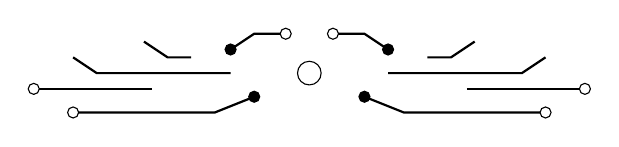
\begin{tikzpicture}
        \coordinate (A) at (0,0);

        \coordinate (B) at (0.7,-0.3);
        \coordinate (C) at (1.2,-0.5);
        \coordinate (D) at (3,-0.5);

        \coordinate (E) at (2,-0.2);        
        \coordinate (F) at (3.5,-0.2);

        \coordinate (G) at (0.3,0.5);
        \coordinate (H) at (0.7,0.5);
        \coordinate (I) at (1,0.3);

        \coordinate (J) at (1.5,0.2);
        \coordinate (K) at (1.8,0.2);
        \coordinate (L) at (2.1,0.4);
        
        \coordinate (M) at (1,0);
        \coordinate (N) at (2.7,0);
        \coordinate (O) at (3,0.2);

        \draw[thick] (B) -- (C) -- (D);
        \draw[thick] (E) -- (F);
        \draw[thick] (G) -- (H) -- (I);
        \draw[thick] (J) -- (K) -- (L);
        \draw[thick] (M) -- (N) -- (O);

        \draw[circle,fill=white] (A) circle (0.15);
        \draw[circle,fill=black] (B) circle (0.07);
        \draw[circle,fill=white] (D) circle (0.07);
        \draw[circle,fill=white] (F) circle (0.07);
        \draw[circle,fill=white] (G) circle (0.07);
        \draw[circle,fill=black] (I) circle (0.07);

        %and now this code mirrored to the other side
        \coordinate (-B) at (-0.7,-0.3);
        \coordinate (-C) at (-1.2,-0.5);
        \coordinate (-D) at (-3,-0.5);

        \coordinate (-E) at (-2,-0.2);
        \coordinate (-F) at (-3.5,-0.2);

        \coordinate (-G) at (-0.3,0.5);
        \coordinate (-H) at (-0.7,0.5);
        \coordinate (-I) at (-1,0.3);

        \coordinate (-J) at (-1.5,0.2);
        \coordinate (-K) at (-1.8,0.2);
        \coordinate (-L) at (-2.1,0.4);

        \coordinate (-M) at (-1,0);
        \coordinate (-N) at (-2.7,0);
        \coordinate (-O) at (-3,0.2);

        \draw[thick] (-B) -- (-C) -- (-D);
        \draw[thick] (-E) -- (-F);
        \draw[thick] (-G) -- (-H) -- (-I);
        \draw[thick] (-J) -- (-K) -- (-L);
        \draw[thick] (-M) -- (-N) -- (-O);

        \draw[circle,fill=black] (-B) circle (0.07);
        \draw[circle,fill=white] (-D) circle (0.07);
        \draw[circle,fill=white] (-F) circle (0.07);
        \draw[circle,fill=white] (-G) circle (0.07);
        \draw[circle,fill=black] (-I) circle (0.07);


       \end{tikzpicture}

\end{center}
\end{document}